    %%
    %% This is file `sample-authordraft.tex',
    %% generated with the docstrip utility.
    %%
    %% The original source files were:
    %%
    %% samples.dtx  (with options: `authordraft')
    %% 
    %% IMPORTANT NOTICE:
    %% 
    %% For the copyright see the source file.
    %% 
    %% Any modified versions of this file must be renamed
    %% with new filenames distinct from sample-authordraft.tex.
    %% 
    %% For distribution of the original source see the terms
    %% for copying and modification in the file samples.dtx.
    %% 
    %% This generated file may be distributed as long as the
    %% original source files, as listed above, are part of the
    %% same distribution. (The sources need not necessarily be
    %% in the same archive or directory.)
    %%
    %% The first command in your LaTeX source must be the \documentclass command.
    \documentclass[sigconf]{acmart}
    
    %%
    %% \BibTeX command to typeset BibTeX logo in the docs
    \AtBeginDocument{%
      \providecommand\BibTeX{{%
        \normalfont B\kern-0.5em{\scshape i\kern-0.25em b}\kern-0.8em\TeX}}}
    
    %% Rights management information.  This information is sent to you
    %% when you complete the rights form.  These commands have SAMPLE
    %% values in them; it is your responsibility as an author to replace
    %% the commands and values with those provided to you when you
    %% complete the rights form.
    \setcopyright{rightsretained}
    \copyrightyear{2019}
    \acmYear{2019}
    \acmDOI{CS460.org}
    
    %% These commands are for a PROCEEDINGS abstract or paper.
    \acmConference[CS460]{CS460: Computer Graphics at UMass Boston}{Fall 2019}{Boston, MA}
    \acmBooktitle{CS460: Computer Graphics at UMass Boston, Fall 2019}
    \acmPrice{1.00}
    \acmISBN{1337}
    
    
    %%
    %% Submission ID.
    %% Use this when submitting an article to a sponsored event. You'll
    %% receive a unique submission ID from the organizers
    %% of the event, and this ID should be used as the parameter to this command.
    %%\acmSubmissionID{123-A56-BU3}
    
    %%
    %% The majority of ACM publications use numbered citations and
    %% references.  The command \citestyle{authoryear} switches to the
    %% "author year" style.
    %%
    %% If you are preparing content for an event
    %% sponsored by ACM SIGGRAPH, you must use the "author year" style of
    %% citations and references.
    %% Uncommenting
    %% the next command will enable that style.
    %%\citestyle{acmauthoryear}
    
    \documentclass{article}
    \usepackage{minted}
    
    %%
    %% end of the preamble, start of the body of the document source.
    \begin{document}
    
    %%
    %% The "title" command has an optional parameter,
    %% allowing the author to define a "short title" to be used in page headers.
    \title{DroidXTK}
    
    %%
    %% The "author" command and its associated commands are used to define
    %% the authors and their affiliations.
    %% Of note is the shared affiliation of the first two authors, and the
    %% "authornote" and "authornotemark" commands
    %% used to denote shared contribution to the research.
    \author{Jared Barresi}
    \email{Jared.Barresi001@umb.edu}
    \affiliation{%
      \institution{University of Massachusetts Boston}
    }
    
    %%
    %% By default, the full list of authors will be used in the page
    %% headers. Often, this list is too long, and will overlap
    %% other information printed in the page headers. This command allows
    %% the author to define a more concise list
    %% of authors' names for this purpose.
    \renewcommand{\shortauthors}{}
    
    %%
    %% The abstract is a short summary of the work to be presented in the
    %% article.
    \begin{abstract}
     DroidXTK is an Android application and framework, of which provides a bridge (in JavaScript) to all the Android API's, for use with the \textcolor{blue}{\hyperlink{http://www.goxtk.com}{XTK framework}}. The Android app is built using the JavaScript platform \textcolor{blue}{\hyperlink{http://www.androidscript.org}{Droidscript}}. Some API "features" implemented include: Button/Slider input, Voice Recognition, Sensor i/o, and many more potential possibilities. The main concept will be to create generalized methods, of which can be used (as is) or easily be extended to provide new functionality in the future.
    \end{abstract}
    
    %%
    %% Keywords. The author(s) should pick words that accurately describe
    %% the work being presented. Separate the keywords with commas.
    \keywords{WebGL, Visualization, Android, JavaScript, XTK, Framework, Droidscript, Developer,API's, Voice-Recognition, Accessibility }
    
    %% A "teaser" image appears between the author and affiliation
    %% information and the body of the document, and typically spans the
    %% page.
    \begin{teaserfigure}
      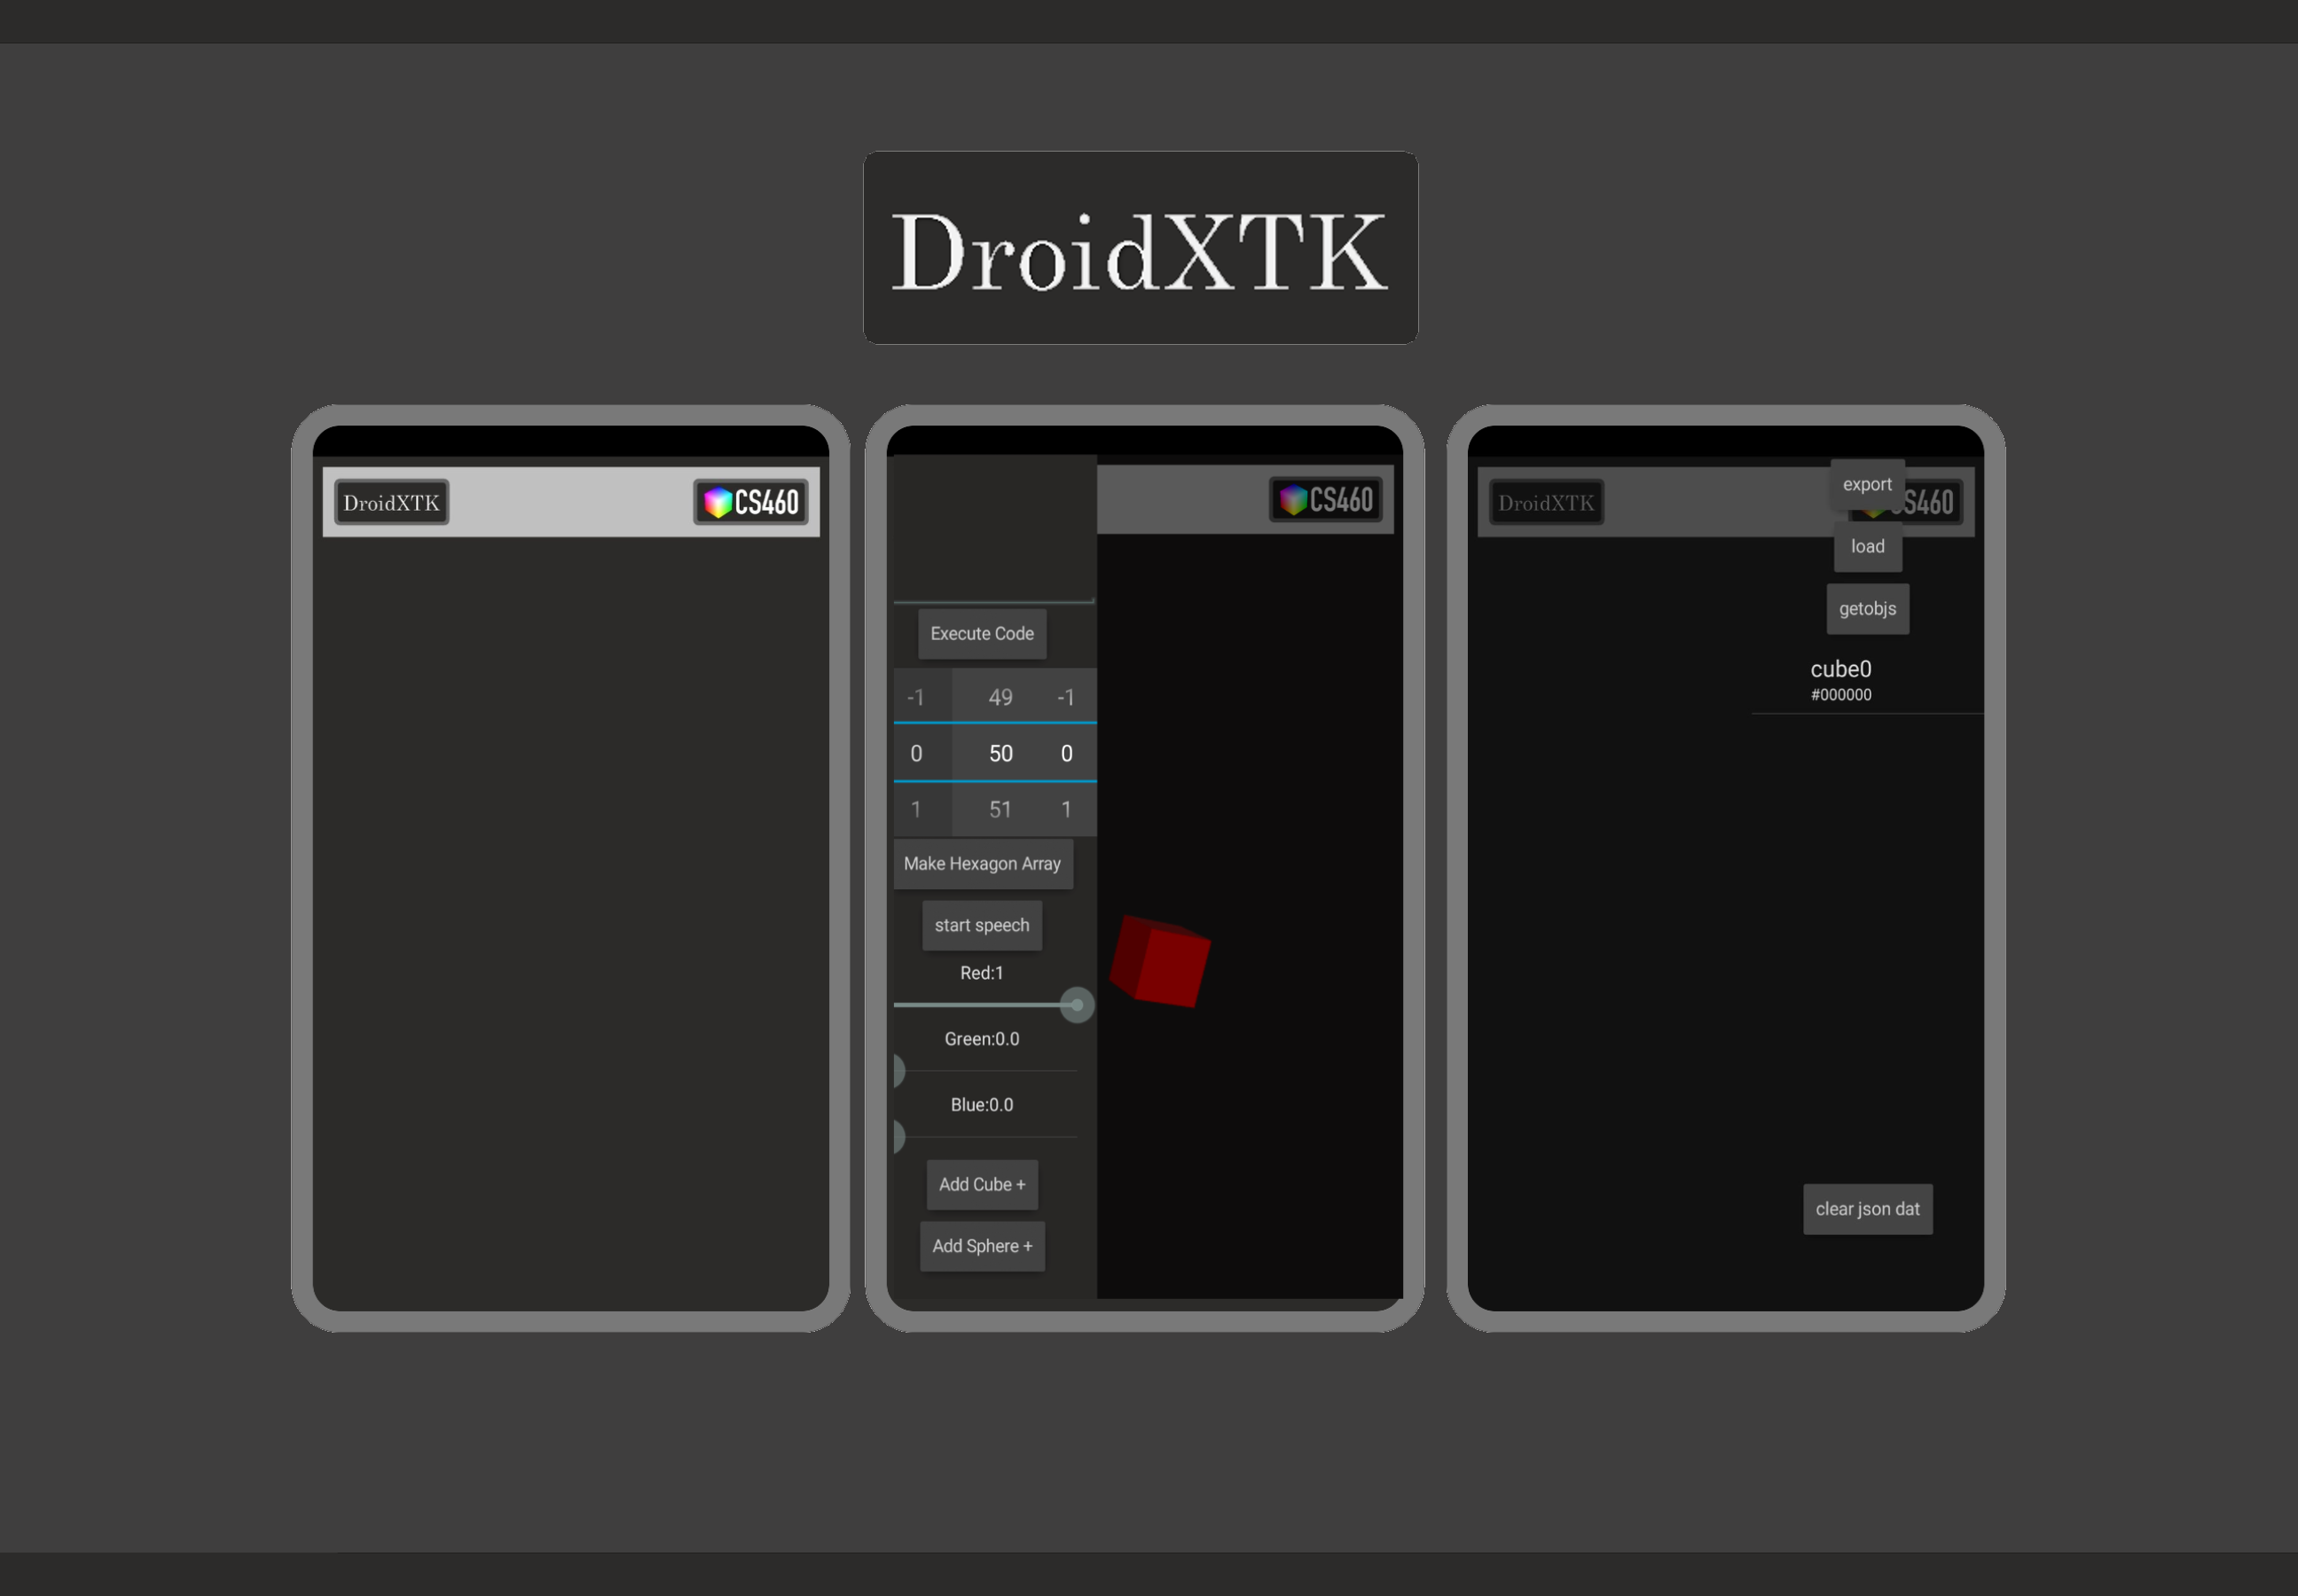
\includegraphics[width=\textwidth]{gfx/droidxtkbanner.png}
      \caption{Create objects, use voice-recognition, and even debug code with the built in web console.  }
      \label{fig:teaser}
    \end{teaserfigure}
    
    %%
    %% This command processes the author and affiliation and title
    %% information and builds the first part of the formatted document.
    \maketitle
    \newpage
    \section{Introduction}
    Using a webview container, you can modify the contents of a page easily via a console. Using an Android framework called Droidscript, you can execute custom-made codes in a webview that has the XTK framework loaded into it.
    
    
    
    \vspace{0.09 cm}
    \textbf{Scripting Engine:}
    
    The DroidScript App contains a scripting engine which allows anyone with a bit of JavaScript knowledge to easily write Apps for their mobile phone or tablet. You can write very simple Apps with just a few buttons, or more complex ones which include dynamic graphical interfaces such as the DroidScript application itself, which is written using the very same engine.
    
    As well as creating graphical interfaces, you have access to Sensors like the Accelerometer, Compass, Light meter or other device components like Wifi, Bluetooth, Camera, GPS, SD Card, SMS, Emails, Internet and more. We're always adding new functionality to the engine, so if you want something added just let us know via email or leave a comment on the forum.
    
    \textbf{Source: } \nolinkurl{ www.androidscript.org}\newline
    \vspace{0.045 cm}
    
    \section{Method}
    
    \textbf{App Object:}
    
    \vspace{0.09 cm}
    The \textbf{app} object is the main driving force behind Droidscript and its easy-to-use JavaScript app development framework. Some of the categories of what the app object extends to include:
    \begin{itemize}
    \item Application Control
    \item Application Information
    \item Bluetooth
    \item Components
    \item Controls
    \item Cross-Application
    \item Database
    \item Debugging
    \item Device Control
    \item Device Information
    \item Dialogs
    \item Files
    \item Graphics
    \item Layouts
    \item Messaging
    \item Network
    \item Sounds
    \item UI Control
    \item User Information
    \end{itemize}
    
    \textbf{source : }\hyperlink{www.androidscript.org}{www.androidscript.org}
    
    \subsection{Implementation}
    \textbf{A "Nested Bridge"}
    \vspace{0.09 cm}
    
    \boxed{
    \boxed{Droidscript} \longrightarrow \boxed{Java} \longrightarrow \boxed{Android API's}}
    \vspace{0.18 cm}
    \newline
    Executes JavaScript code on live HTML/JavaScript, in an Android webview container. XTK code bridge created in JavaScript to using Droidscript framework to develop methods.
    \vspace{0.09 cm}
    
    \textbf{Android Controls: }
    
    \begin{minted}{javascript}
    //controls to initialize methods
    bexec = app.CreateButton("load");
    btnClearJsonData = app.CreateButton("clear json dat");
    btnCube = app.CreateButton("Add Cube +");
    btnDebug = app.CreateButton("Execute Code");
    btnobjlst = app.CreateButton("getobjs");
    btnspch = app.CreateButton("start speech");
    btnSphere = app.CreateButton("Add Sphere +");
    btnwpcg = app.CreateButton("export");
    createHexagon = app.CreateButton("Make Hexagon Array");
    //data entry fields to store values to apply to XTK objects
    edt = app.CreateTextEdit("",-1 ,0.18,"mono");
    labelBlue = app.CreateText("Blue:0.0");
    labelGreen = app.CreateText("Green:0.0");
    labelRed = app.CreateText("Red:0.0");
    //layouts to hold the prior objects
    layDebug = app.CreateLayout("linear","VTop");
    layDebug.AddChild(btnCube);
    layDebug.AddChild(btnDebug);
    layDebug.AddChild(btnspch);
    layDebug.AddChild(btnSphere);
    layDebug.AddChild(createHexagon);
    layDebug.AddChild(edt);
    layDebug.AddChild(layRGB);
    layDebug.AddChild(layXYZPos);
    layObjDebug = app.CreateLayout("linear","VTop");
    layObjDebug.AddChild(bexec);
    layObjDebug.AddChild(btnClearJsonData);
    layObjDebug.AddChild(btnobjlst);
    layObjDebug.AddChild(btnwpcg);
    layObjDebug.AddChild(objlist);
    layRGB = app.CreateLayout("linear","Vertical");
    layRGB.AddChild(labelBlue);
    layRGB.AddChild(labelGreen);
    layRGB.AddChild(labelRed);
    layRGB.AddChild(skbBlue);
    layRGB.AddChild(skbGreen);
    layRGB.AddChild(skbRed);
    layXYZPos = app.CreateLayout("linear","Horizontal");
    layXYZPos.AddChild(txtXPos);
    layXYZPos.AddChild(txtYPos);
    layXYZPos.AddChild(txtZPos);
    //list to store and track objects created
    objlist = app.CreateList(",",0.45,0.63);
    //More controls to change properties post-running
    skbBlue = app.CreateSeekBar(-1,-1);
    skbGreen = app.CreateSeekBar(-1,-1);
    skbRed = app.CreateSeekBar(-1,-1);
    \end{minted}
    
    \newpage
    
    \section{Milestones}
    
    \subsection{Milestone 1}
    \textit{Date:   Wed Dec 11 19:04:09 2019 -0500}\newline
    Created a working production version, calling it DroidXTK.
    
    \subsection{Milestone 2}
    \textit{Date:   Mon Dec 9 15:22:42 2019 -0500}\newline
    Added android app project + resources - reorganized assets
    
    \subsection{Milestone 3}
    
    \textit{Date:   Mon Dec 9 10:24:52 2019 -0500}\newline
    Wrote initial codes and prototypes.
    
    \subsection{Milestone 4}
    
    \textit{Date:   Sat Nov 23 09:12:17 2019 -0500}\newline
    Created scripts that modify webview through app.Execute() (Executes code in webview in Droidscript)
    
    \subsection{Milestone 5}
    
    \textit{Date:   Thu Nov 21 20:45:06 2019 -0500}\newline
    Added links and repositories for project ideas.
    
    \subsection{Milestone 6}
    \textit{Date:   Thu Nov 21 11:25:40 2019 -0500}\newline
    Added final project directory, created symlinks to resources for project potentials, and created link folder to store relevant pages.
    
    \subsection{Challenges}
    Getting voice recognition to work correctly, as it required numerous if/else and switch statements to properly process the code (without it "breaking" the rest of the code).
    
    \section{Results}
    
    \vspace{0.09 cm}
    
    \textbf{XTK Bridge Method:}
    
    \begin{minted}{javascript}
    function dsx()
    {
    dsx.objectsarray = [];
    var objlst = [];
    //create new xtk obj counter
    this.counter = function (name)
    {
    //counter name
    var cname = "counter_" + name
    //counter as new variable (integer counter)
    this.cnt = cname;
    //set count to 0
    cname = 0;
    //return counter object
    return cname;
    }
    this.cube = function (name, x, y, z, r, g, b)
    {
    dsx.setobj(name, x, y, z, r, g, b);
    var code = ""
    code += (name + " = new X.cube(); \n ")
    code += (name + ".center" + " = 
    [" + x + "," + y + "," + z + "]; \n ")
    code += (name + ".color" + " = 
    [" + r + "," + g + "," + b + " ]; \n ")
    code += ("r.add( " + name + "); \n ")
    code += ("r.render(); \n ");
    return code;
    }
    
    ...
    
    this.getobjlst = function ()
    {
    return dsx.objectsarray;
    }
    
    ...
    
    dsx.writeAsJson = function (path, obj)
    {
    app.WriteFile(path, JSON.stringify(obj));
    }
    
    dsx.readAsJson = function (path)
    {
    if (app.FileExists(path))
    {
    return JSON.parse(app.ReadFile(path));
    }
    app.ShowPopup(path + " does not exist");
    return undefined;
    }
    
    ...
    \end{minted}
    
    \section{Conclusions}
    Had a great working prototype app, that could create several different geometry types, of which you could track their properties, change them, and create additional ones through use of my main xtk() method. The bridge created through my methods, enabled relatively unbounded access to the Android API's and frameworks, allowing them to exchange data back and forth efficiently.
    
    %%
    %% REFERENCES
    %%
    \bibliographystyle{ACM-Reference-Format}
    \biblioht
    \bibliography{references}
    
    [1] \textbf{XTK Toolkit:   }   \hyperlink{http://goxtk.com}{http://goxtk.com/}
    
    [2] \textbf{Dave Smart, Droidscript Framework:    }   \hyperlink{http://droidscript.org/}{http://droidscript.org/}
    
    \end{document}
    \endinput
